\chapter{Model Structure}\label{Ch:Model}

\section{Generator}

As we mentioned earlier, baseline structure mainly used in this project is Cycle-GAN. The Cycle-GAN consists of two GAN models, which learn to translate images from one domain to the other, one direction per each respectively. 

The first architecture we selected as generators is the \emph{Residual Network}~\cite{resnet}. Being published in 2015, The skip connection of ResNet is considered one of most important idea in the field of deep learning. What the skip connection is doing is nothing more than copy early features of layer and paste it to later layers, and known to help the training process of neural networks a lot. There are many explanation why this helps, one of the most significant one is that it makes the optimization problem that deep networks faces by making loss function to be optimized over smoother manifold~\cite{li2018visualizing}.

The ResNet consists of small modules called `residual module' which has two 3 by 3 convolutions and one skip connection. This topology makes ResNet model to be stacked deep without making optimization too difficult. While this structure make it suitable for classification and also for other purposes, we decided to use U-net for our case because it is known to keep details in images better than ResNet does.

Fig~\ref{FIG:unet} shows overall structure of U-net. While the U-net also features the skip connection as the ResNet, U-net differs from it in that it has skip connection from symmetrical shape. The skip connections connecting early layers with the later layers transport the low-level features to the high-level layers which significantly reduces spatial infomation loss and ensures feedback on internal structures of both inputs and outputs.

\begin{figure}[ht]
    \begin{center}
    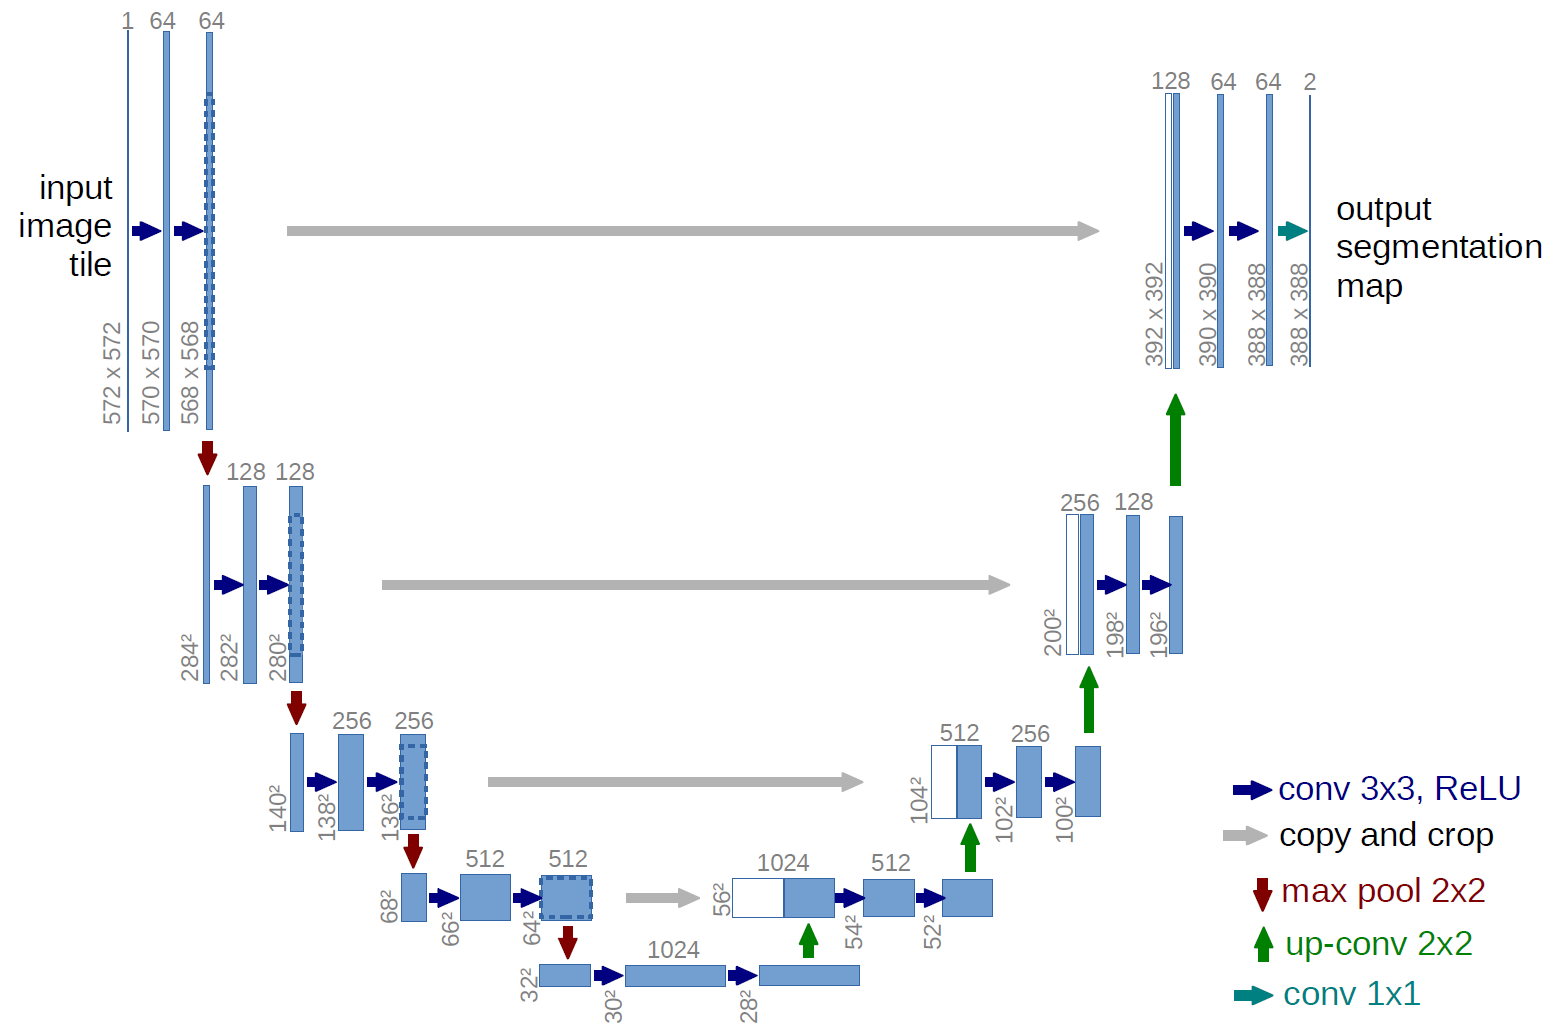
\includegraphics[scale=0.2]{Graphics/u-net-architecture.png}
    \end{center}
    \caption{Structure of original U-net~\cite{unet}.}\label{FIG:unet}
\end{figure}

While the original U-net only used central part of images abandoning the boundary features, we used input padding on the boundary inputs to keep images to be invariant in size. In addition, different from the original U-net, we replaced the transposed-convolution with nearest-neighbor upsample and convolution of kernel size 3, which are known to prevent output images from generating checkerboard-like artifacts by removing the overlap between filters~\cite{odena2016deconvolution}.

\section{Discriminator}

For the discriminators we used the 70 by 70 PatchGAN discriminator with instance normalizations, which is same as the original CycleGAN article. For stability of the train process, we added some noise to the real / fake label and flipped the labels once in a hundred.

Finally, we utilized 'grouped convolutions~\cite{Grouped}' to the bottleneck(most deepest part of U-net) with 4 groups, which makes convolution operation happens separately on the 4 separated groups of intermediate features in networks. For more detailed information about model structure, the reader can refers to our published code.

\endinput

